%%%%%%%%%%%%%%%%%%%%%%%%%%%%%%%%%%%%%%%%%
% University Assignment Title Page 
% LaTeX Template
% Version 1.0 (27/12/12)
%
% This template has been downloaded from:
% http://www.LaTeXTemplates.com
%
% Original author:
% WikiBooks (http://en.wikibooks.org/wiki/LaTeX/Title_Creation)
%
% License:
% CC BY-NC-SA 3.0 (http://creativecommons.org/licenses/by-nc-sa/3.0/)
% 
% Modified for COSC480/490 by:
% Lech Szymanski (8/3/18)
%
% Modified for Eden's COSC385 report. (09/2025)

\documentclass[12pt]{article}
\usepackage[draft]{cosc4x0style}
\usepackage{float}
\usepackage{tikz}
\usepackage[edges]{forest}
\usetikzlibrary{shapes,arrows,positioning,shapes.multipart,arrows.meta,fit,backgrounds}

% To compile the final version of the report (which will remove all the todo content)
%\usepackage{cosc4x0style}

% Specify project code 480 or 490
\papercode{385}

% Your project title
\title{Talking in French Like Academia\\\large Machine Learning Powered Verlan Identification}

% Your name
\author{Yitian \textsc{Li}}
\studentid{4556502}

% Names of your supervisors, separated by line break '\\'
\supervisors{
  Dr. Lech \textsc{Szymanski} \\
  Dr. Veronica \textsc{Liesaputra}
}

% Date, change the \today to a set date if you want to be precise
\reportdate{\today}

\begin{document}


\maketitle

\begin{abstract}
something.
\end{abstract}

\section{Introduction}
\subsection{Context and Motivation}

Since the early 19th century, the French people have started to talk using verlan. Just like Pig Latin\footnote{\url{en.wikipedia.org/wiki/Pig_Latin}} exists in English culture, verlan is an unusual and creative form of \textit{argot} (slang) that is formed by flipping the syllables around in a word.\footnote{In fact, the word \textit{verlan} is a verlan from the word \textit{l'inver} (the inversion).}\cite{rajabov2025,bach2018} 
Time flies, verlan has become more and more popular, and it is now widely used amongst teens and young people in francophone societies\footnote{Such as France, Belgium, Switzerland, Luxembourg, and Canada.}\cite{evolutionverlan}. Examples of verlan can be as follows:

\begin{flushleft}
\small
\begin{itemize}
  \item bite = bi + te \(\rightarrow\) te + bi \(\rightarrow\) tebie (penis)
  \item shit = shi + t \(\rightarrow\) t + shi \(\rightarrow\) teuchi\cite{evolutionverlan}
  \item bonjour = bon + jour \(\rightarrow\) jour + bon \(\rightarrow\) jourbon (greetings)
\end{itemize}
\end{flushleft}

\noindent In real-life conversations, such can be used as in the example sentences below:

\begin{flushleft}
\small
\begin{itemize}
  \item \textit{Le graff géant représente une tebie pixel art.}\\(The giant graffiti depicts a pixel art penis.)
  \item \textit{Il a du bon teuchi du bled.}\\(He's got some good shit from the countryside.)
  \item \textit{Un p'tit\footnote{Standard spelling: petit.}jourbon et tout le monde sourit.}\\(A quick hello and everyone smiles.)
\end{itemize}
\end{flushleft}

Indeed, verlan can be formed with different original languages, not only French, but also English and other languages. However, it always follows the same rule of flipping syllables, although, for better pronunciation reasons, certain minor amendments such as dropping unnecessary letters and applying accents (e.g., é, è) can be used from time to time\cite{rajabov2025}. Besides, due to the universal trait of slang being used more often phonetically instead of written, verlan users tend to spell them differently when writing them down. As technology develops, this has been occurring more frequently than ever in daily texting\cite{rua2005}.

Thinking internationally, when people are communicating with translators, it is possible that slang in their mother language can be brought to the conversation, which could be tricky for translators to translate\cite{hajiyeva2025}. Using translators such as DeepL\footnote{\url{www.deepl.com}} and Google Translate\footnote{\url{translate.google.com}} to translate sentences that contain verlan from French to English can be a specific example to prove this. Furthermore, although both of the translators above are using Machine Learning (ML) for translation, their results of translating verlans are not ideal\cite{deepl2020, wu2016}. For example, when attempting to translate the sentence above, \textit{Le graff géant représente une tebie pixel art.}, both Google Translate\ref{fig:google_verlan} and DeepL\ref{fig:deepl_verlan} cannot translate the word \textit{tebie} correctly. Specifically, for DeepL, there is no desired translation as \textit{penis} in its alternative word list for \textit{tebie}\ref{fig:deepl_alt_text}.

\begin{figure}[H]
\centering
\includegraphics[width=0.8\textwidth]{figures/google_verlan.png}
\caption{\label{fig:google_verlan}Google Translate cannot translate the verlan \textit{tebie} correctly.}
\end{figure}

\begin{figure}[H]
\centering
\includegraphics[width=0.8\textwidth]{figures/deepl_verlan.png}
\caption{\label{fig:deepl_verlan}DeepL cannot translate the verlan \textit{tebie} correctly.}
\end{figure}

\begin{figure}[H]
\centering
\includegraphics[width=0.3\textwidth]{figures/deepl_alt_text.png}
\caption{\label{fig:deepl_alt_text}No desired translation for verlan \textit{tebie} in DeepL's alternative word list.}
\end{figure}

Thus, a question shall naturally arise: Can we improve translators' performance in translating slang by improving the ML model? The answer is undoubtedly `yes' in an era where artificial intelligence research is expanding rapidly. Researchers have been making progress in identifying slang using ML\cite{pei2019slang} and, moreover, in translating noisy text, of which slang is a part\cite{michel2018mtnt}. 

But what about verlan? There is no known ongoing or completed research on identifying \textit{such} slang or their translations\footnote{Until September 2025.}, nor does a proper dataset exist. The only work similar to this is an assignment published at the University of Toronto\footnote{\url{https://uoft-csc413.github.io/2022/assets/assignments/PA03.pdf}}, asking students to train a Neural Machine Translation (NMT) model to transform standard English into Pig Latin. It is not only the other way around; instead of identifying Pig Latin and transforming it back to standard English, it is also more of an example for students to practice using NMT than a discussion on its identification and translation. Shouldn't we do something?

This report aims to change that.

\subsection{Objective}

The purpose of the project is to create two verlan datasets: one functioning as a dictionary, containing the verlan words and their normalised standard French equivalents; the other a dataset of sentences that contain verlan, paired with the same sentences containing normalised words, with labels indicating whether a sentence contains verlan. After that, the project embeds and classifies verlan using Large Language Models (LLMs) and analyses the results.

\begin{figure}[H]
\centering
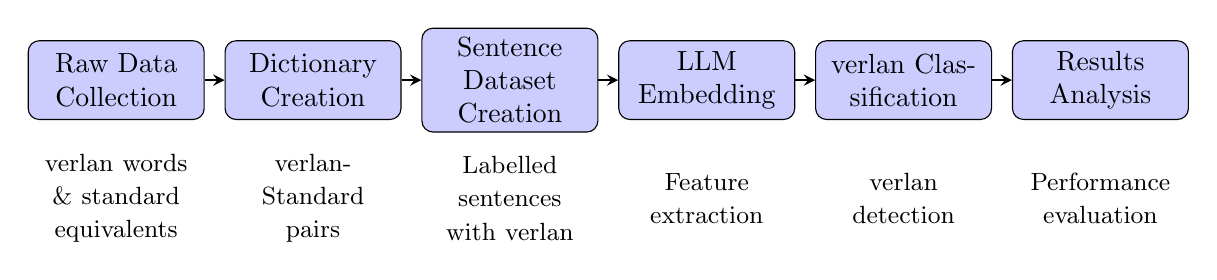
\begin{tikzpicture}[
    node distance=2.5cm,
    auto,
    block/.style={rectangle, draw, fill=blue!20, text width=2cm, text centered, rounded corners, minimum height=1cm},
    arrow/.style={thick,->,>=stealth}
]

% Define nodes from left to right
\node [block] (data) {Raw Data Collection};
\node [block, right of=data] (dict) {Dictionary Creation};
\node [block, right of=dict] (sentences) {Sentence Dataset Creation};
\node [block, right of=sentences] (embedding) {LLM Embedding};
\node [block, right of=embedding] (classification) {verlan Classification};
\node [block, right of=classification] (analysis) {Results Analysis};

% Draw arrows
\draw [arrow] (data) -- (dict);
\draw [arrow] (dict) -- (sentences);
\draw [arrow] (sentences) -- (embedding);
\draw [arrow] (embedding) -- (classification);
\draw [arrow] (classification) -- (analysis);

% Add labels below nodes
\node [below of=data, node distance=1.5cm, text width=2cm, text centered] {\small verlan words \& standard equivalents};
\node [below of=dict, node distance=1.5cm, text width=2cm, text centered] {\small verlan-Standard pairs};
\node [below of=sentences, node distance=1.5cm, text width=2cm, text centered] {\small Labelled sentences with verlan};
\node [below of=embedding, node distance=1.5cm, text width=2cm, text centered] {\small Feature extraction};
\node [below of=classification, node distance=1.5cm, text width=2cm, text centered] {\small verlan detection};
\node [below of=analysis, node distance=1.5cm, text width=2cm, text centered] {\small Performance evaluation};

\end{tikzpicture}
\caption{\label{fig:pipeline}A visulisation of the objectives.}
\end{figure}

With the purpose above, the report contributes to the linguistics and the AI researchers two verlan datasets, for dictionary making or LLMs training. The report also evaluates how good we can achieve the identification of verlan with ML, to benefit machine translation in the future.

The code and the unannotated, un peer-reviewed dataset developed as part of the project are released under openlicences and aligns with open science best practices, with the usage of a version controlled software development platform (GitHub)\footnote{\url{github.com/greateden/verlan-Identification-Normalisation}}. The annotated, peer-reviewed dataset will be published shortly after this report, aiming by the end of 2025.

\section{Background}
\subsection{A Living Verlan}

Vivienne Véla, a former scholar from Université Paris 8, poetically captured one of Verlan's most important traits: it pursues confusion instead of clarity\cite{mela1991verlan}. One reason is that it is widely used among lower-class people, drug users, gangs, or those in jail. Thus, making the context unidentifiable is important\;---\;certain phenomena such as reverlanisation (flipping the Verlan again if it becomes too popular) and truncation are therefore applied. However, although Verlan is used for concealing meaning, it still follows certain rules. The most general rule is syllabic reversal, as mentioned in the introduction chapter of this report.

Specifically, to delve into the linguistic rules, Véla pointed out that the analytic model proposed by Kaye and Lowenstamm provides the best description\cite{kaye1984syllabicite}. The syllable can be disassembled into \textit{attaque} (onset), \textit{rime} (rhyme), \textit{noyau} (nucleus), and \textit{coda}. For example, here is a representation of the word \textit{garder}, IPA\footnote{International Phonetic Alphabet, \url{https://en.wikipedia.org/wiki/International_Phonetic_Alphabet}} [garde].

\begin{figure}[H]
\centering
\begin{forest}
for tree={
  grow=south,
  parent anchor=south,
  child anchor=north,
  align=center,
  edge={-latex},
  l sep=10pt,
  s sep=18pt,
  font=\itshape
}
[{\textbf{garder}}
  [{$S_1$}
    [attaque
      [g, font=\normalfont]
    ]
    [rime
      [noyau
        [a, font=\normalfont]
      ]
      [coda
        [r, font=\normalfont]
      ]
    ]
  ]
  [{$S_2$}
    [attaque
      [d, font=\normalfont]
    ]
    [rime
      [noyau
        [e, font=\normalfont]
      ]
    ]
  ]
]
\end{forest}
\end{figure}

It has two syllables, $S_1$ and $S_2$. To create the Verlan form, we follow the permutation equation below:

\begin{equation}\label{eq:verlan-perm}
  (S_1 S_2) \rightarrow (S_2 S_1)
\end{equation}

After the permutation, we obtain the Verlan form of \textit{garder} as \textit{degar}, represented below.

\begin{figure}[H]
\centering
\begin{forest}
for tree={
  grow=south,
  parent anchor=south,
  child anchor=north,
  align=center,
  edge={-latex},
  l sep=10pt,
  s sep=18pt,
  font=\itshape
}
[{\textbf{degar}}
  [{$S_2$}
    [attaque
      [d, font=\normalfont]
    ]
    [rime
      [noyau
        [e, font=\normalfont]
      ]
    ]
  ]
  [{$S_1$}
    [attaque
      [g, font=\normalfont]
    ]
    [rime
      [noyau
        [a, font=\normalfont]
      ]
      [coda
        [r, font=\normalfont]
      ]
    ]
  ]
]
\end{forest}
\end{figure}

Notably, the permutation occurs only at the syllable level (i.e., between $S_1$ and $S_2$); it does not affect the internal structure of each syllable tree, although in some cases, certain letters (such as \textit{e}) might be dropped after permutation. That said, the example above is not an exhaustive explanation of forming a Verlan. To avoid confusing the readers, this report suggests that this example perfectly illustrates its regular rule. For further details, readers are advised to consult Véla's paper.

With such a sub-word permutation, researchers can not only discuss it within the linguistic realm, but it is also intriguing for computer scientists to explore how machines, such as LLMs, perceive this kind of difference. Just as Véla describes Verlan\;---\;ambiguous, sometimes violent, sometimes amazing, and always vivid.


\subsection{Detecting Slang}

To the best of our knowledge, there is no existing computational research\footnote{As of September 2025.} on the \textit{detection} of Verlan\;---\;this particular form of French slang. However, there are a few scholars who have included Verlan in their research\cite{zurbuchen2024, podhorna2020rapcor, mekki2021tremolo, panckhurst202088milsms}. Yet, these studies commonly included Verlan as a type of slang in their datasets or corpora. Moreover, they did not specifically focus on how to detect this particular type of slang, but rather approached it in a broader sense\;---\;they created slang datasets that contain Verlan, and some of them employed computational approaches to detect such slang.

Fortunately, there are several papers related to computational slang detection, and their approaches could contribute to Verlan detection to a large extent\cite{pei2019slang, sun2024informal, slangornot2024, wu2018slangsd}. These studies are not limited to French but also cover other Indo-European languages\footnote{For example, English, German, and Russian. For more information, please refer to: \url{https://en.wikipedia.org/wiki/Indo-European_languages}.}.

Therefore, regarding the history of Verlan detection, this report first generalises the task as slang detection, and then discusses possible methods that could be implemented for Verlan identification, in order to provide readers with a general and useful background.

\subsubsection{1910s-2016: A Super-Condensed History of Slang Detection}

The background of traditional slang detection often leverages fuzzy-matching methods. Two main methods were introduced and widely cited: Soundex, a phonetic indexing system for names introduced by Russell in 1918, and the edit-distance-based spelling-correction method introduced by Levenshtein in 1966\cite{russell1918soundex, levenshtein1966}. Afterwards, scholars introduced more algorithms, such as Philips's Metaphone and Double Metaphone, which improved on Russell's Soundex; Kukich's methods for detecting and correcting spelling; Sproat's normalisation of Non-Standard Words (NSW); and Aw et al.'s phrase-based Machine Translation (MT) approach for standardising SMS messages\cite{philips1990metaphone,philips2000doublemetaphone, kukich1992techniques,sproat2001normalization,aw2006phrase}. While these are not directly slang-detection research, over time their methodology became increasingly related to slang\;---\;some slang can be treated as misspelling or NSW, and people frequently use slang in text messages.


\subsubsection{2016-2019: Dictionary Search}

The easiest way we can think of dealing with slang is to use a dictionary\;---\;just like how we look up a word that we do not know. The pros and cons are highly similar to consulting a dictionary. It is fast (if using a digital one) and accurate. On the other hand, because it is purely fixed data, it only works with existing words and thus cannot identify newly invented ones.

Examples of existing slang dictionaries include SlangNet, SlangSD, and SLANGZY\cite{dhuliawala2016slangnet, wu2018slangsd, gupta2019slangzy}. As for French slang dictionaries, we have, for example, \textit{Dictionnaire du chilleur}\cite{dictionnaire2024chilleur}. Specifically for Verlan, the report identifies several online dictionaries, including \textit{Dictionnaire Interactif du Verlan}\footnote{\url{https://ecoleng.com/verlan-comprendre-argot-francais-parler/dictionnaire-interactif-du-verlan}}, Wiktionary\footnote{\url{https://en.wiktionary.org/wiki/Category\%3AVerlan}}, and \textit{Dictionnaire Verlan}\footnote{\url{https://zlang.fandom.com/fr/wiki/Dictionnaire_Verlan}}.

With these existing dictionaries, implementing a tool to identify Verlan should be straightforward. However, two major issues limit the possibility of directly using these dictionaries for Verlan identification: they lack comprehensive coverage, and some are fan-made, which neither captures the full extent of this slang nor guarantees accuracy. Licensing for certain dictionaries could also be a concern.

Although dictionaries have the drawbacks mentioned above, they remain essential resources for implementing LLM-based approaches, as discussed later. Consequently, new dictionaries continue to be produced.

\subsubsection{Meanwhile, for Fuzzy Search}

The 2010s belonged to social media and research on user-generated text. Representative work includes Beaufort et al.'s hybrid finite-state framework for SMS normalisation, Han and Baldwin's lexical normalisation for Twitter, and the W-NUT shared tasks on Twitter message normalisation\cite{beaufort2010hybrid, han2011lexical, baldwin2015shared}.

While these works are not directly about slang recognition, they provided immensely useful background for the research specifically on slang that followed.

\subsubsection{2020-2025: Fuzzy Search + Slang Corpus = BOOM}

In the 2020s, everyone tended to check what could be done with Machine Learning (ML) for this task, using Natural Language Processing (NLP). Researchers started to apply NLP to slang detection. Wilson's paper used two million entries from \textit{Urban Dictionary}, with terms, definitions, examples, and tags\cite{urban2020embeddings}. They pre-processed the dataset with techniques like lowercasing and removal of punctuation, followed by training a fastText\footnote{A library for learning of word embeddings and text classification created by Facebook's AI Research (FAIR) lab.} skip-gram for 10 epochs with a 300-dimensional vector space. Using a fastText classifier, they analysed properties such as sentiment and sarcasm. For evaluation, they used accuracy, precision, recall, and F1 score.

Notably, the report has found two theses highly related to this project, \textit{Slang or not?} and \textit{Toward Informal Language Processing}\cite{sun2024informal,slangornot2024}. Both created their own datasets that were manually annotated and validated. The former compared the performance of traditional ML (SVM\footnote{Support Vector Machine, \url{https://en.wikipedia.org/wiki/Support_vector_machine}}-linear with TF-IDF\footnote{\url{https://en.wikipedia.org/wiki/Tf\%E2\%80\%93idf}} + n-grams), Convolutional Neural Network (CNN)\footnote{\url{https://en.wikipedia.org/wiki/Convolutional_neural_network}} / Bidirectional Long-Short Term Memory (BiLSTM)\footnote{\url{https://en.wikipedia.org/wiki/Long_short-term_memory}} with Bidirectional Encoder Representations from Transformers (BERT)\footnote{\url{https://en.wikipedia.org/wiki/BERT_(language_model)}} embeddings, Transformer models (e.g., BERT-large-uncased), and Large Language Models (LLMs) (GPT-4o and GPT-4o-mini), finding that a fine-tuned Transformer performed best. The latter compared traditional baselines, Language Models (LMs), and LLMs. 

\subsubsection{Detecting Verlan?}
The results from the last section provide this report with a clear guideline regarding Verlan identification. They have absorbed and adapted the historical development of slang detection into a modern, up-to-date framework. Building upon these insights, this report argues that BERT and contemporary LLMs represent the most effective tools for the Verlan detection task.

\section{Datasets}
\subsection{The Separated Structures}
As of the time of writing, there are no published Verlan datasets. Thus, this report has created two datasets: one is a lookup table mapping words in Verlan to their standard French forms, named \textit{GazetteerEntries} (hereafter \textit{the dictionary}); the other contains example sentences for the words appearing in the table, both in Verlan and in standard French, with three entries per form, named \textit{Sentences}. The general reasons for having two datasets are:

\begin{enumerate}
  \item To separate rules and learning signals. The dictionary works as a lookup and a baseline for rule-matching: it provides word mappings, word variants, etc., whilst the sentences dataset is for detection and evaluation and illustrates \textit{how} verlan appears in context. If mixed together, the model will not be able to distinguish tokens as dictionary knowledge or usage.
  \item To improve reusability. The dictionary can be used independently on any corpus for rule-based verification, while the sentences dataset can be updated separately to add more community examples without modifying the dictionary, supporting modularisation of the pipeline.
  \item For a cleaner evaluation. The dictionary can serve as a baseline while the sentences dataset can be split for training and testing, making results easier to interpret.
\end{enumerate}

Generally speaking, the separation of the datasets can potentially make the model and the experiments clearer, explainable, and easy to extend. They could also contribute to LLM training and corpus creation in the future.

\subsection{Visualisation of the Datasets}

Figure~\ref{fig:dataset-structure} presents the attributes in the datasets and highlights how they relate to each other.

\begin{figure}[p]
\centering
\tikzset{
  table/.style={
    draw,
    rounded corners=2pt,
    thick,
    align=left,
    inner sep=5pt,
    fill=white,
    minimum width=7.8cm
  },
  header/.style={
    fill=black!5,
    text=black,
    font=\bfseries,
    inner xsep=8pt,
    inner ysep=6pt,
    rounded corners=2pt,
    draw
  },
  field/.style={font=\ttfamily\small, align=left},
  note/.style={font=\scriptsize, text=black!60},
  legend/.style={
    draw,
    rounded corners=2pt,
    align=left,
    inner sep=5pt
  },
  connect/.style={-Latex, very thick, black!35}
}
\begin{tikzpicture}[node distance=0.8cm]

\node[header, minimum width=7.8cm] (ghead) {GazetteerEntries};
\node[table, below=0pt of ghead, anchor=north] (gtable) {%
  \begin{tabular}{@{}l@{}}
    {\bfseries Attributes (name: type)} \\[2pt]
    \texttt{gazetteer\_id}: \textit{integer} \\
    \texttt{verlan\_form}: \textit{text} \\
    \texttt{standard\_form}: \textit{text} \\
    \texttt{pos}: \textit{enum} (\texttt{noun}, \texttt{verb}, \texttt{adj}, \dots) \\
    \texttt{is\_phrase}: \textit{boolean} \\
    \texttt{tier}: \textit{enum} (\texttt{gold}|\texttt{silver}|\texttt{bronze}) \\
    \texttt{origin\_lang}: \textit{text} \\
    \texttt{notes}: \textit{text} \\[2pt]
  \end{tabular}
};

\node[note, below=2pt of gtable.south] (gnote) {Lexicon \& mapping for rule-based match + normalisation.};

\node[header, minimum width=9.2cm, below=0.8cm of gnote] (shead) {Sentences};
\node[table, below=0pt of shead, anchor=north, minimum width=8.6cm] (stable) {%
  \begin{tabular}{@{}l@{}}
    {\bfseries Attributes (name: type)} \\[2pt]
    \texttt{sentence\_id}: \textit{integer} \\
    \texttt{text}: \textit{text} \\
    \texttt{reference}: \textit{url/text} \\
    \texttt{accessed\_on}: \textit{date} (ISO~8601) \\
    \texttt{domain}: \textit{text} (e.g., \texttt{rap}, \texttt{sms}, \texttt{forum}, \dots) \\
    \texttt{quality\_flag}: \textit{enum} (\texttt{gold}|\texttt{silver}|\texttt{bronze}) \\
    \texttt{has\_verlan}: \textit{boolean} \\[2pt]
  \end{tabular}
};

\node[note, below=2pt of stable.south] (snote) {Context corpus for detection \& evaluation.};

\draw[connect] (gtable.south west) .. controls +(-0.6,-1.0) and +(-0.6,1.0) .. node[left, text=black!50, pos=.55]{\scriptsize lookup / match} (stable.north west);
\draw[connect] (gtable.south east) .. controls +(0.6,-1.0) and +(0.6,1.0) .. node[right, text=black!50, pos=.45]{\scriptsize normalise to \texttt{standard\_form}} (stable.north east);

\node[legend, below=0.8cm of snote] (legend) {%
  \textbf{Legend}\\
  \texttt{name}: \textit{type}\\
  \textit{integer}=\#; \textit{text}=string; \textit{boolean}=\texttt{true|false}\\
  \textit{enum}=fixed set of values; \textit{date}=YYYY-MM-DD
};

\begin{scope}[on background layer]
  \node[draw=black!10, rounded corners=3pt, fit=(ghead) (gtable) (gnote) (shead) (stable) (snote) (legend), inner sep=6pt] {};
\end{scope}
\end{tikzpicture}
\caption{\label{fig:dataset-structure}Overview of the GazetteerEntries lookup table and the Sentences corpus, including their key attributes.}
\end{figure}


\subsection{The Creations}

As mentioned in Section~2.2.2, this report first checked and scraped sources that were available and had researcher-friendly copyright policies. Among those mentioned, \textit{Dictionnaire Verlan} and Wiktionary contributed the most in terms of quantity. However, as they are not curated or officially published, their quality is not guaranteed. Moreover, many entries do not provide example sentences, which makes the creation of the sentences corpus harder.

\subsubsection{Sampling}
Although there is no clear estimate of the overall quantity of Verlan, after searching, scraping, and combining, this report compiled a total of 1{,}086 Verlan items, though some are merely spelling variants of the same word. For example, \textit{foncédé} and \textit{foncedé}\footnote{Verlan of \textit{défoncé}, often translated as \textit{high (on drugs)} in English.} are counted separately as two entries; so are \textit{keus} and \textit{keuss}\footnote{Verlan of \textit{sec}, translated as \textit{dry} in English.}. Notably, there are around 150 entries for which the report did not find their standard form; thus they have been categorised as \textit{bronze} regarding their quality. To the best of our knowledge, the dictionary we have created contains the largest number of Verlan entries among the public dictionaries we could find.

After creating the dictionary, the report searched for and scraped usage examples online to create the sentences corpus. The report also used Artificial Intelligence (AI) tools\;---\;specifically, ChatGPT Deep Research\footnote{\url{https://openai.com/index/introducing-deep-research/}}\;---\;for sentence scraping. The results for sentences with a verifiable reference have been marked as \textit{gold} quality; those without a verifiable reference have been marked as \textit{silver} quality. For items for which the report could not find example sentences, we prompted ChatGPT-o3\footnote{\url{https://en.wikipedia.org/wiki/OpenAI_o3}} to generate example sentences; these results have been marked as \textit{bronze} quality. All results have been reviewed by the author of this report and are intended to undergo annotation in the future.

\subsubsection{Quality Tiers}

To provide readers with a clearer understanding of the tier/quality schema introduced in this report, we have created a table for clarity:

\begin{table}[H]
\centering
\caption{Quality tiers of the Verlan datasets.}
\begin{tabular}{c|l|l}
\hline
\textbf{Tier} & \textbf{Definition} & \textbf{Source} \\
\hline
Gold   & Verified with public reference & Public reference (URL/citation) \\
Silver & Plausible sentence without verifiable source & Scraped / semi-auto \\
Bronze & LLM-generated and manually reviewed & ChatGPT-o3 \\
\hline
\end{tabular}
\label{tab:verlan_tiers}
\end{table}


\subsection{Final Dataset}

At the time of writing, the datasets are not yet officially finalised. Although the structure of the two datasets is as shown in Section~3.2, in the dictionary dataset this report did not invest much effort in annotating the original language of the Verlan items; the \textit{note} column is also scarcely used. In the sentences corpus, the \textit{accessed\_on} and \textit{domain} columns are also scarcely annotated. 

The main reason is that these columns were not used in the implementations. In fact, this report only used \textit{gazetteer\_id}, \textit{verlan\_form}, and \textit{standard\_form} in the dictionary, and \textit{sentence\_id}, \textit{text}, and \textit{has\_verlan} in the sentences corpus. To us, the remaining columns are primarily for publishing the datasets and for potential advanced experiments in the future.

\section{Experiments}

After constructing and verifying the datasets, the report has conducted a series of experiments to 

\subsection{Experimental Settings}
\subsubsection{Model Architectures and Specifications}
%
\subsubsection{Evaluation Methodology}
\subsubsection{Lookup Baseline}

\subsection{Results and Analyses}
\subsubsection{Embedding Space Visulisation}
\subsubsection{}
\subsubsection{}

\subsection{Conclusions and Limitations}


% Besides, identifying the same word with different spelling or declensions is also a hurdle. although we do have those fuzzy search algorithms, the report is not sure whether 

% mention that because we need to train LLMs, having verlans embedding in sentences is important, whilst the report wanna make good use of the benefits of dictionary search, so the report has made two datasets -- on just purly Verlan - Standard French mapping, the other is Verlan sentences.


\section{Discussion and Outlook}


\newpage

%The environment \thebibliography produces a list of references; such list will be titled "References". A parameter inside braces, 9 in the example, indicates the number of entries to be added; this parameter can not be greater than 99.

%To create a bibliography entry the command \bibitem is used. A parameter inside braces is set to label this entry and can later be used as identifier for this reference. After the closing brace the text with the name of the author, the book title, publisher and so on is entered. 

%Any choice of citation style is acceptable as long as you are consistent.

\begin{thebibliography}{9}

\bibitem{rajabov2025} 
Radjabov, Ruslan Rajabmurodovich. \textit{Understanding "verlan" in the French Language}. 
Web of Scientist: International Scientific Research Journal, vol. 6, no. 3, 2025, pp. 368-372. 
Available at: \url{https://webofjournals.com/index.php/3/article/view/3264}.

\bibitem{bach2018} 
Bach, Xavier. \textit{Tracing the origins of verlan in an early nineteenth century text}. 
Journal of French Language Studies, vol. 28, no. 1, 2018, pp. 1-18. 
Cambridge University Press. doi:10.1017/S0959269516000221.

\bibitem{evolutionverlan} 
Olivier Sécardin. \textit{Évolution du verlan, marqueur social et identitaire, comme reflet de la langue et de la société françaises}. 
Synergies Europe, no. 3, 2008, pp. 223-232. 
Available at: \url{https://journal.lib.uoguelph.ca/index.php/synergies/article/download/1037/1859?inline=1}.

\bibitem{rua2005} 
Rúa, Paula López. “Shortening Devices in Text Messaging.” 
\textit{Journal of Computer-Mediated Communication}, vol. 10, no. 4, July 2005. 
Wiley. doi:10.1111/j.1083-6101.2005.tb00268.x.

\bibitem{hajiyeva2025}  
Hajiyeva, Bulbul. “Translating Idioms and Slang: Problems, Strategies, and Cultural Implications.”  
Acta Globalis Humanitatis et Linguarum, vol. 2, no. 2, 2025, pp. 284-293. doi:10.69760/aghel.025002123.  

\bibitem{deepl2020} 
DeepL. “DeepL Translator translates texts using artificial neural networks. These networks are trained on many millions of translated texts.” 
\textit{DeepL Blog}, 2020. Available at: \url{https://www.deepl.com/en/blog/how-does-deepl-work}.

\bibitem{wu2016} 
Wu, Yonghui, et al. “Google's Neural Machine Translation System: Bridging the Gap between Human and Machine Translation.” 
arXiv preprint arXiv:1609.08144, 2016. Available at: \url{https://arxiv.org/abs/1609.08144}.

\bibitem{michel2018mtnt}
Michel, Paul, and Graham Neubig. “MTNT: A Testbed for Machine Translation of Noisy Text.”
\textit{Proceedings of EMNLP}, 2018. Available at: \url{https://aclanthology.org/D18-1050/}.

\bibitem{zurbuchen2024}
Zurbuchen, Lucas, and Rob Voigt.  
\textit{A Computational Analysis and Exploration of Linguistic Borrowings in French Rap Lyrics}.  
In *Proceedings of the 62nd Annual Meeting of the Association for Computational Linguistics — Student Research Workshop (ACL SRW 2024)*, 2024, pp. 200-208.  
DOI: 10.18653/v1/2024.acl-srw.27.  

\bibitem{podhorna2020rapcor}
Podhorná-Polická, Alena.  
\textit{RapCor, Francophone Rap Songs Text Corpus}.  
In *Proceedings of the Fourteenth Workshop on Recent Advances in Slavonic Natural Language Processing (RASLAN 2020)*, 2020, pp. 95-102.  
Available at: \url{https://nlp.fi.muni.cz/raslan/raslan20.pdf#page=95}.  % (no DOI found)

\bibitem{mekki2021tremolo}
Mekki, Jade; Lecorvé, Gwénolé; Battistelli, Delphine; Béchet, Nicolas.  
\textit{TREMoLo-Tweets: A Multi-Label Corpus of French Tweets for Language Register Characterization}.  
In *Proceedings of the International Conference on Recent Advances in Natural Language Processing (RANLP 2021)*, Held Online, INCOMA Ltd., Sep 1-3, 2021, pp. 950-958.  
DOI: 10.26615/978-954-452-072-4\_108.  

\bibitem{panckhurst202088milsms}
Panckhurst, Rachel; Lopez, Cédric; Roche, Mathieu.  
\textit{A French text-message corpus: 88milSMS. Synthesis and usage}.  
Corpus [En ligne], 20 | 2020 (mis en ligne le 28 janvier 2020).  
DOI: 10.4000/corpus.4852.  

\bibitem{pei2019slang}
Pei, Zhengqi, Zhewei Sun, and Yang Xu.  
\textit{Slang Detection and Identification}.  
In *Proceedings of the 23rd Conference on Computational Natural Language Learning (CoNLL 2019)*, Hong Kong, China, 2019, pp. 881-889.  
Available at: \url{https://aclanthology.org/K19-1082/}.  % (ACL Anthology entry — no DOI)

\bibitem{sun2024informal}
Sun, Zhewei, Qian Hu, et al.  
\textit{Toward Informal Language Processing: Knowledge of Slang in Large Language Models}.  
In *Proceedings of the 2024 Conference of the North American Chapter of the Association for Computational Linguistics (NAACL 2024)*, 2024.  
DOI: 10.18653/v1/2024.naacl-long.94.  

\bibitem{slangornot2024}
Anonymous.  
\textit{Slang or Not? Exploring NLP Techniques for Slang Detection Using the SlangTrack Dataset}.  
ACL ARR (OpenReview) submission, December 2024 (ACL ARR 2024 December).  
Available at: \url{https://openreview.net/forum?id=bISO3DD8sU}.

\bibitem{wu2018slangsd}
Wu, Tianyang; Morstatter, Fred; Liu, Huan; et al.  
\textit{SlangSD: Building, Expanding, and Using a Sentiment Dictionary of Slang Words for Short-Text Sentiment Classification}.  
Language Resources and Evaluation (2018).  
DOI: 10.1007/s10579-018-9416-0.  

\bibitem{dhuliawala2016slangnet}
Dhuliawala, Shehzaad; Kanojia, Diptesh; Bhattacharyya, Pushpak.  
\textit{SlangNet: A WordNet like Resource for Slang Words}.  
In: Proceedings of the Tenth International Conference on Language Resources and Evaluation (LREC 2016).  
Portorož, Slovenia (2016).  
Available at: \url{https://www.cse.iitb.ac.in/~pb/papers/lrec16-slangnet.pdf}.

\bibitem{wu2018slangsd}
Wu, Tianyang; Morstatter, Fred; Liu, Huan; et al.  
\textit{SlangSD: Building, Expanding, and Using a Sentiment Dictionary of Slang Words for Short-Text Sentiment Classification}.  
Language Resources and Evaluation (2018).  
DOI: 10.1007/s10579-018-9416-0.  

\bibitem{gupta2019slangzy}
Gupta, Vishal; Rani, Rekha; et al.  
\textit{SLANGZY: A Slang Word Recognition System for Hindi-English Code-Mixed Social Media Text}.  
In: Proceedings of the 6th Workshop on South and Southeast Asian Natural Language Processing (WSSANLP 2019).  
Kolkata, India (2019).  
Available at: \url{https://aclanthology.org/K19-1082.pdf}.

\bibitem{dictionnaire2024chilleur}
Parent, Philippe; Parent, André.  
\textit{Dictionnaire du chilleur}.  
Éditions Somme toute (2024).  
ISBN: 9782925124351.  

\bibitem{mela1991verlan}
Méla, Vivienne.  
\textit{Le verlan ou le langage du miroir}.  
Langages, No. 101, Les javanais (Mars 1991), pp. 73–94.  
Published by Armand Colin.  
Available at: \url{https://www.jstor.org/stable/23906698}.

\bibitem{kaye1984syllabicite}
Kaye, Jonathan D.; Lowenstamm, Jean.  
\textit{De la syllabicité}.  
In: Dell, François; Hirst, Daniel; Vergnaud, Jean-Roger (eds.), \textit{Forme sonore du langage}.  
Hermann, Paris (1984), pp. 123–159.  
Available at: \url{https://archive.org/details/formesonoredulangage}.

\bibitem{russell1918soundex}
Russell, Robert C.; Odell, Margaret K.  
\textit{Soundex system of indexing names}.  
U.S. Patent 1,261,167, filed June 3, 1918, and issued April 2, 1918.  
Available at: \url{https://patents.google.com/patent/US1261167A/en}.

\bibitem{levenshtein1966}
Levenshtein, Vladimir I.  
\textit{Binary codes capable of correcting deletions, insertions, and reversals}.  
Soviet Physics Doklady, vol. 10, no. 8, 1966, pp. 707-710.  
Available at: \url{https://nymity.ch/sybilhunting/pdf/Levenshtein1966a.pdf}.

\bibitem{philips1990metaphone}
Philips, Lawrence.
\textit{Hanging on the Metaphone}.
Computer Language (1990).
Available at: \url{https://aspell.net/metaphone/}.

\bibitem{philips2000doublemetaphone}
Philips, Lawrence.
\textit{The Double Metaphone Search Algorithm}.
C/C++ Users Journal (June 2000).
Available at: \url{https://xlinux.nist.gov/dads/HTML/doubleMetaphone.html}.

\bibitem{kukich1992techniques}
Kukich, Karen.
\textit{Techniques for automatically correcting words in text}.
ACM Computing Surveys (1992).
DOI: 10.1145/146370.146380.

\bibitem{sproat2001normalization}
Sproat, Richard; Black, Alan W.; Chen, Stanley; Kumar, Shankar; Ostendorf, Mari; Richards, Christopher.
\textit{Normalization of non-standard words}.
Computer Speech \& Language, 15(3):287–333 (2001).
DOI: 10.1006/csla.2001.0169.

\bibitem{aw2006phrase}
Aw, AiTi; Zhang, Min; Xiao, Juan; Su, Jian.
\textit{A Phrase-Based Statistical Model for SMS Text Normalization}.
Proceedings of the COLING/ACL 2006 Main Conference Poster Sessions (2006), pages 33–40.
Available at: \url{https://aclanthology.org/P06-2005/}.

\bibitem{beaufort2010hybrid}
Beaufort, Richard; Roekhaut, Sophie; Cougnon, Louise-Amélie; Fairon, Cédrick.
\textit{A Hybrid Rule/Model-Based Finite-State Framework for Normalizing SMS Messages}.
Proceedings of the 48th Annual Meeting of the Association for Computational Linguistics (ACL 2010).
Available at: \url{https://aclanthology.org/P10-1079.pdf}.

\bibitem{han2011lexical}
Han, Bo; Baldwin, Timothy.
\textit{Lexical Normalisation of Short Text Messages: Makn Sens a \#twitter}.
Proceedings of the 49th Annual Meeting of the Association for Computational Linguistics: Human Language Technologies (ACL-HLT 2011), pages 368–378.
Available at: \url{https://aclanthology.org/P11-1038/}

\bibitem{baldwin2015shared}
Baldwin, Timothy; de Marneffe, Marie Catherine; Han, Bo; Kim, Young-Bum; Ritter, Alan; Xu, Wei.
\textit{Shared Tasks of the 2015 Workshop on Noisy User-generated Text: Twitter Lexical Normalization and Named Entity Recognition}.
Proceedings of the Workshop on Noisy User-generated Text (W-NUT 2015).
DOI: 10.18653/v1/W15-4319.

\bibitem{urban2020embeddings}
Urban Dictionary Embeddings.
\textit{Urban Dictionary Embeddings for Slang NLP Applications}.
LREC / ACL Anthology (2020).
Available at: \url{https://aclanthology.org/2020.lrec-1.586/}.

\bibitem{sun2024knowledge}
Sun, X.; et al.
\textit{Knowledge of Slang in Large Language Models}.
Proceedings of the 2024 Annual Conference of the North American Chapter of the Association for Computational Linguistics (NAACL-Long 2024).
Available at: \url{https://aclanthology.org/2024.naacl-long.94/}.




\end{thebibliography}


% Activate the appendix
% from now on sections are numerated with capital letters
\appendix

\renewcommand{\thesection}{Appendix \Alph{section}}

\section{Some extra things}

If you have anything more to add such as:
\begin{itemize}
\item not essential details - things that might be too much for first time reading, or could be distracting from the main points...but are still important for reproducibility or deeper understanding
\item work that was done in the project but doesn't go with the main work, or detracts/is not essential for the main narrative.  
\end{itemize}

\section{Aims and Objectives}

\textbf{Interim report only!} -- you do not need to include this appendix in the final report.  However, in your interim the last appendix should include your original Aims and Objectives, and, if the things have changed, the revised Aims and Objectives. If you used the \LaTeX{} template provided for your Aims and objectives document, just copy the \verb$\paragraph{Aims}$ and \verb$\paragraph{Objectives}$ sections and paste them here.

\subsection*{Original}

\paragraph{Aims}
Here you are describing the term goal of the project. What do you want to achieve by the end?  What is the ultimate goal of this work?  For example, the primary aim of this document is to have students produce suitable aims and objectives for their COSC480/490 project. While the aims and objectives document is not an assessed deliverable, a clear definition of what is to be done, and a bit of planning of how it is to be accomplished is paramount to the project's success. It is important to establish the scope of the project.

\paragraph{Objectives}
Objectives list the milestones that you need to achieve in order to achieve the projects aim(s). It's a rough plan for what needs to happen in what order. It's best to list the objectives in bullet point form. For many projects the structure to these objectives might follow the following pattern (objective names are just examples -- you can have different objective names):    
\begin{itemize}[noitemsep]
\item background reading; going through the literature; learning about the research field;
\item setting up of some kind of system for the project; getting the environment for experiments working;
\item conducting preliminary experiments; implementation of a basic/simple approach; producing base case results;
\item trying method 1; recording the results;
\item trying method 2; recording the results.
\end{itemize}

\subsection*{Revised}

\paragraph{Aims}
Here you are describing the term goal of the project. What do you want to achieve by the end?  What is the ultimate goal of this work?  For example, the primary aim of this document is to have students produce suitable aims and objectives for their COSC480/490 project. While the aims and objectives document is not an assessed deliverable, a clear definition of what is to be done, and a bit of planning of how it is to be accomplished is paramount to the project's success. It is important to establish the scope of the project.

\paragraph{Objectives}
Objectives list the milestones that you need to achieve in order to achieve the projects aim(s). It's a rough plan for what needs to happen in what order. It's best to list the objectives in bullet point form. For many projects the structure to these objectives might follow the following pattern (objective names are just examples -- you can have different objective names):    
\begin{itemize}[noitemsep]
\item background reading; going through the literature; learning about the research field;
\item setting up of some kind of system for the project; getting the environment for experiments working;
\item conducting preliminary experiments; implementation of a basic/simple approach; producing base case results;
\item trying method 1; recording the results;
\item trying method 2; recording the results.
\end{itemize}


\end{document}
